\documentclass[11pt,a4paper]{article}
\usepackage[margin=2.2cm]{geometry}
\usepackage[T1]{fontenc}
\usepackage{lmodern,microtype}
\usepackage{graphicx,booktabs,tabularx,float,caption,xcolor,enumitem,amsmath,array,multirow}
\usepackage[hidelinks]{hyperref}
\graphicspath{{../figures/}{../../results/plots/}}
\captionsetup{font=small,labelfont=bf}
\setlist{itemsep=2pt,topsep=4pt}
\newcolumntype{R}{>{\raggedleft\arraybackslash}X}
\makeatletter % float-only pages: stack floats from the top instead of spreading them out
\setlength{\@fptop}{0pt}\setlength{\@fpsep}{14pt}\setlength{\@fpbot}{0pt plus 1fil}
\makeatother

\title{\textbf{Processing and Visualising Large DEMs on a Laptop}\\[4pt]
\large Progress Report, Phase 5: Interactive Viewing with Debounced Pan/Zoom and Prefetch}
\author{Team GeoGuessers \quad|\quad Spatial Informatics\\[4pt]
Swayam Goyal (2024111012) \quad Siddharth Choudhary (2024111021)\\
Yakkala Viswanadha Kartikeya (2024111033)}
\date{}

\begin{document}
\maketitle

\begin{abstract}
\noindent
Phases 2--4 showed that terrain processing on a laptop is bound by decoding and memory, not by arithmetic, and that
a derivative computed on demand from a pyramid level costs the same few milliseconds at every zoom level. This
phase builds a viewer on that result and measures it. A tile server computes slope, aspect, hillshade and
roughness products for fixed $512\times512$ tiles on demand. Its foreground workers run on the performance cores
and prefetch on the efficiency cores, with block and tile caches and cancellation. A browser viewer pans and zooms
continuously: it commits a zoom once, after a trailing debounce, and prefetches the eight neighbouring views. A
QGIS plugin computes any dragged box. We replayed 17 seeded interaction traces against a fresh server in 24
configurations, 1{,}068 runs in all. With prefetch, 98--100\% of the tiles entering the view while panning are
already in the browser, at up to two view widths per second. The debounce cuts the tiles the server renders per
zoom gesture from 62 to 19, and the first exact tile follows the debounce within 63--71\,ms. Prefetch does not slow
the foreground: on identical tiles the server's 95th-percentile latency is 90\,ms with prefetch and 95\,ms without,
because prefetch stops whenever the user acts. Notched-wheel traces set the debounce default to 150\,ms. A real
browser (headless Chrome) reproduces the simulated client's request counts and timings within 10\%.
\end{abstract}

\section{Objective}
The meeting asked for a viewer that works like a map: pan and zoom freely, compute only what is in view at the
resolution the screen needs, and prefetch what the user will probably look at next. The goals come from the team's
Phase 5 specification; the internal design is ours. The questions are:
\begin{enumerate}
  \item Can on-the-fly computation keep up with continuous pan and zoom on one laptop?
  \item Does a trailing debounce on zoom cut the server's work, and what delay does it add?
  \item Does prefetching the neighbouring views make panning seamless without slowing the visible tiles?
  \item Which settings (debounce, prefetch policy, worker pools, core placement, caches) should be the defaults?
\end{enumerate}
Two gates were set in advance: prefetch must not raise foreground p95 latency by more than 10\%, and the debounce
must reduce server tiles per zoom gesture while keeping the first frame within 100\,ms of the debounce.

\section{The system}
\begin{table}[H]
\centering\small
\caption{Components built in this phase (all in the repository).}
\label{tab:system}
\begin{tabularx}{\linewidth}{>{\raggedright\arraybackslash}p{2.6cm}X}
\toprule
Component & Design \\
\midrule
Tile engine & Fixed $512\times512$ tile lattice per pyramid level, aligned to the COG's $512^2$ blocks, with a 1-cell halo.
One tile is rendered on one thread by GIL-free Numba kernels, so tiles run in parallel (5.4$\times$ on 8 threads).
Decoded blocks are cached and shared by neighbouring tiles; encoded tiles are cached too. Output is 8-bit palette
PNG. Modes: \emph{auto} (the level's own cells, E5 error), \emph{exact} (full resolution, averaged), \emph{precomputed}. \\
Scheduler & Foreground and background queues. Foreground workers are pinned to the 12 performance-core threads and
background workers to the 8 efficiency cores. Identical requests share one job; a foreground request promotes a
queued prefetch job. A newer generation of a session supersedes older work. Cancellation is checked between
read, kernel and encode. Prefetch does not start while foreground work is pending, and pauses when memory is low. \\
Server & FastAPI: tiles, overview, \texttt{POST /view} (a box as PNG or GeoTIFF), session generations, stats. Every
tile reports its queue, read, decode, kernel, colour-map and encode times. A closed connection cancels its job
(median 37\,ms). \\
Web viewer & Each frame draws the needed level's tiles, falling back to a coarser or finer cached level and then
the overview. Zoom commits once, after a trailing debounce; pan requests new tiles at once. After a commit the eight
neighbouring views are prefetched, in the direction of travel first, at most two at a time. Shift + drag zooms to
a box. \\
QGIS plugin & Drag a box; the server's GeoTIFF result is added as a styled layer. A full-resolution box is identical
to \texttt{gdaldem}'s slope of the full-resolution DEM. \\
\bottomrule
\end{tabularx}
\end{table}

\section{Method}
\paragraph{Virtual client.} A Python port of the viewer's policy (camera, level choice, browser cache, debounce,
generations, aborts, prefetch) reads the same policy file as the browser. It replays a trace in real time against
the live server, over HTTP/1.1 with at most six connections (a browser's limit per server), and simulates 60\,Hz
frames. Python's default event-loop clock on Windows advances in 15.6\,ms steps, so the client runs its own loop on
the high-resolution clock.

\paragraph{Traces.} Seeded, for a $1600\times900$ view:
\begin{itemize}
  \item \textbf{Pans:} straight and reversing pans at 0.5, 1 and 2 view widths per second (5\,s), and a random walk.
  \item \textbf{Zoom bursts:} 60\,Hz wheel bursts of 0.3, 1 and 2\,s, in and out, over 1--3 levels.
  \item \textbf{Notched wheel:} ten discrete notches 30--150\,ms or 120--300\,ms apart.
  \item \textbf{Zoom-pan:} 10\,s of alternating bursts and pans.
  \item \textbf{Box:} three nested box zooms from the whole map to full resolution.
\end{itemize}

\paragraph{Protocol.} One factor at a time around the defaults, 24 configurations; 1 warm-up and 5 measured runs
for every configuration and trace. Each run:
\begin{itemize}
  \item starts a new server process with empty caches, and loads the first view and its prefetch ring before the
  trace clock starts;
  \item reads the server's counters at the start and end of the trace, and samples memory every 50\,ms.
\end{itemize}
The data is the Chamoli 2\,m DEM (pyramid levels 0--6), with hillshade, unless stated.

\paragraph{Metrics.}
\begin{itemize}
  \item \emph{Pan hit rate}: share of tiles already cached when they enter the view.
  \item \emph{Blank area-time}: share of view area $\times$ frames not drawn from the needed level's own tiles.
  \item \emph{TTFF}: last wheel tick to the first frame showing a tile of the committed level.
  \item \emph{Complete}: last tick to the first frame in which every visible tile is drawn.
  \item \emph{Server tiles per gesture}: foreground jobs finished or cancelled mid-render.
  \item \emph{Prefetch precision}: prefetched tiles later drawn, as a share of all prefetched tiles.
  \item \emph{Foreground p95}: measured at the client and on the server.
\end{itemize}

\section{Results}
\subsection{Defaults}
\begin{table}[!htbp]
\centering\small
\caption{Default policy on every trace (median of 5 runs; debounce 200\,ms, the sweep's base). TTFF and Complete
(ms) for zoom traces include the debounce; Tiles/gest. = server foreground tiles per zoom gesture.}
\label{tab:base}
\footnotesize\setlength{\tabcolsep}{2pt}
\begin{tabular*}{\linewidth}{@{\extracolsep{\fill}}lrrrrrr}
\toprule
Trace & Fg req. & Prefetched & Hit rate & TTFF & Complete & Tiles/gest. \\
\midrule
pan-line 0.5/1/2 & 0 / 0 / 2 & 175 / 313 / 333 & 1.00 / 1.00 / 0.99 & & & \\
pan-reverse 0.5/1/2 & 0 / 0 / 5 & 73 / 128 / 443 & 1.00 / 1.00 / 0.98 & & & \\
pan-walk & 0 & 290 & 1.00 & & & \\
zoom in 0.3/1/2\,s & 20 / 15 / 20 & & & 272 / 273 / 289 & 325 / 325 / 358 & 20 / 15 / 20 \\
zoom out 0.3/1/2\,s & 18 / 20 / 12 & & & 269 / 264 / 257 & 321 / 314 / 276 & 18 / 20 / 12 \\
zoom-pan & 36 & 128 & 1.00 & 206 & 206 & 7.2 \\
box & 35 & 125 & & 64 & 127 & \\
\bottomrule
\end{tabular*}
\end{table}

On-the-fly computation keeps up (Table~\ref{tab:base}):
\begin{itemize}
  \item \textbf{Pans} need almost no foreground requests: the prefetch ring already holds the tiles.
  \item \textbf{Zooms:} the first exact tile arrives 57--89\,ms after the commit and the full view 76--158\,ms after
  it.
  \item \textbf{Box zoom} shows its first exact tile 64\,ms after the animation ends.
  \item \textbf{Cost:} the server never needed more than 982\,MiB. Prefetch used about 3 CPU-seconds of the
  efficiency cores per 5\,s pan.
\end{itemize}
Figure~\ref{fig:timeline} shows what the viewer draws during zoom-pan: the needed level's own tiles cover the view
except for a few hundred milliseconds after each zoom-in, when cached coarser tiles stand in.

\begin{figure}[!htbp]
\centering
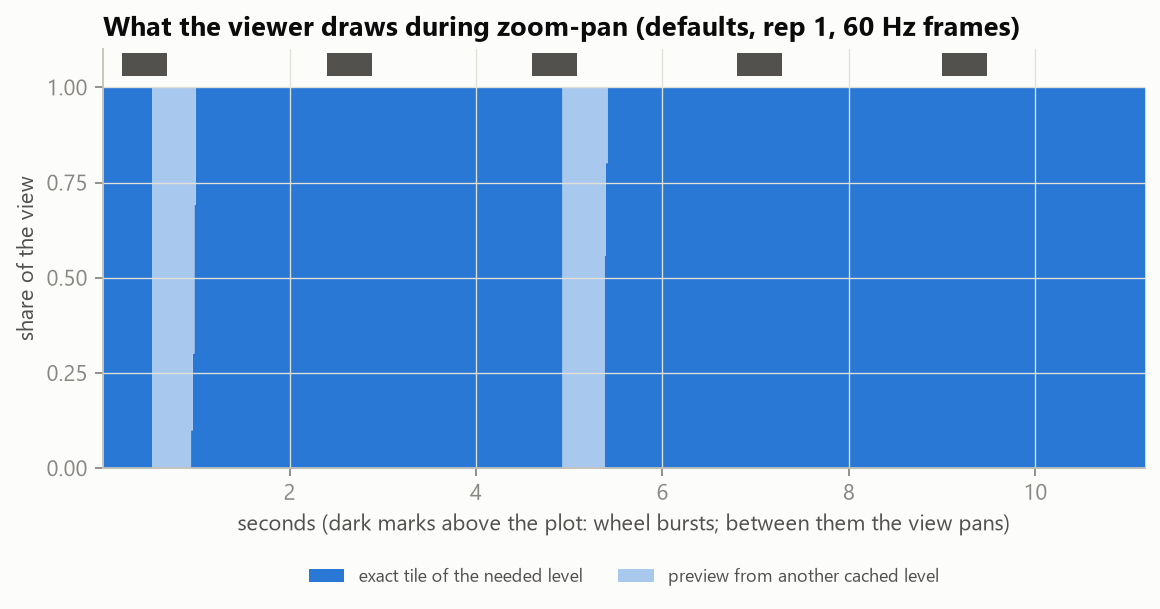
\includegraphics[width=0.82\linewidth]{e6_timeline.png}
\caption{Share of the view drawn from the needed level's own tiles (dark) or from another cached level (light),
60\,Hz frames, during zoom-pan with the defaults.}
\label{fig:timeline}
\end{figure}

\subsection{Debounce (gate 2)}
\begin{figure}[!htbp]
\centering
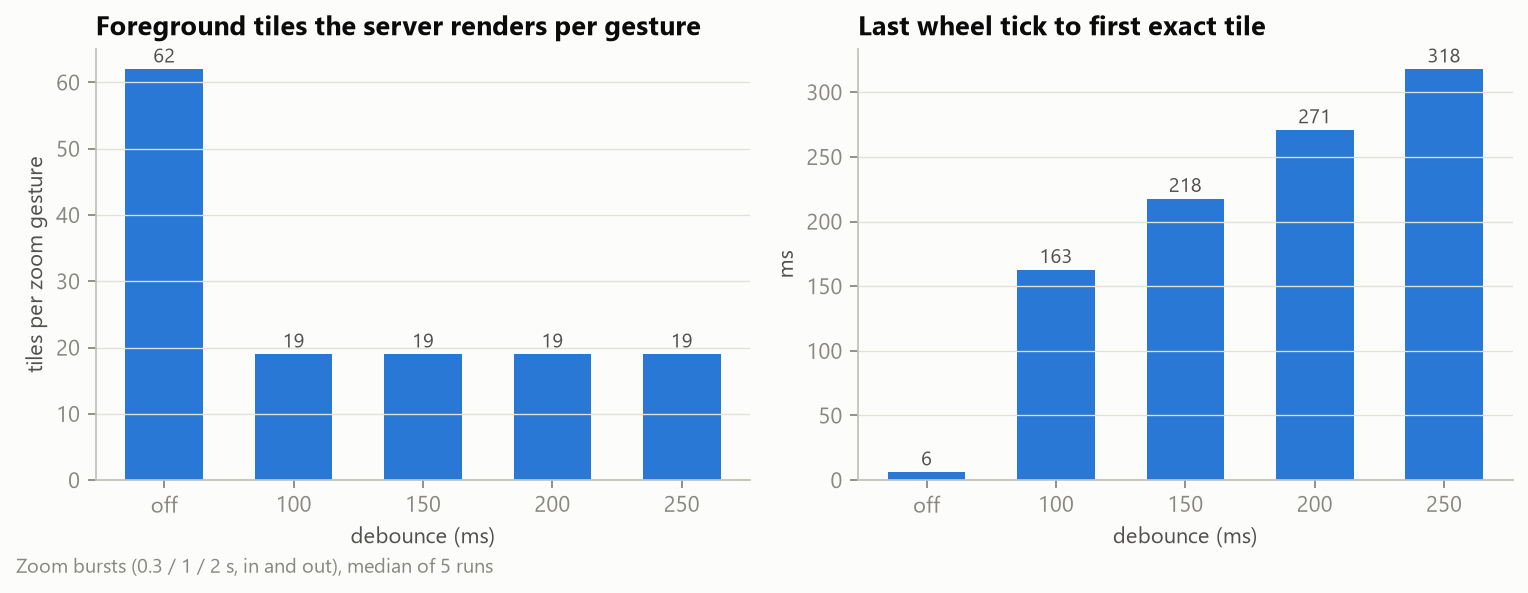
\includegraphics[width=\linewidth]{e6_debounce.png}
\caption{Zoom bursts at 60\,Hz: foreground tiles the server renders per gesture, and time from the last tick to the
first exact tile, against the debounce.}
\label{fig:debounce}
\end{figure}

\begin{table}[!htbp]
\centering\small
\caption{Server foreground tiles per zoom gesture and delay, by debounce (median of runs).}
\label{tab:debounce}
\begin{tabularx}{\linewidth}{lRRRRR}
\toprule
Debounce & 60\,Hz bursts & Notched 30--150\,ms & Notched 120--300\,ms & TTFF $-$ debounce, bursts (ms) & TTFF, bursts (ms) \\
\midrule
off (every tick) & 62 & 36 & 48 & -- & 6 \\
100\,ms & 19 & 36 & 48 & 63 & 163 \\
\textbf{150\,ms (new default)} & 19 & \textbf{15} & \textbf{39} & 68 & 218 \\
200\,ms & 19 & 15 & 39 & 71 & 271 \\
250\,ms & 19 & 15 & 39 & 68 & 318 \\
200\,ms + forced commit at 500\,ms & 35 & 30 & 39 & 62 & 262 \\
\bottomrule
\end{tabularx}
\end{table}

\begin{itemize}
  \item \textbf{Without a debounce} every tick commits, up to 121 times in a 2\,s burst. The server renders a median
  of 62 foreground tiles per gesture and cancels 4--19 of them mid-render.
  \item \textbf{With a debounce} it renders 19, \textbf{3.3$\times$ fewer}, and the first exact tile arrives
  63--71\,ms after the debounce fires. The gate passes (Table~\ref{tab:debounce}, Figure~\ref{fig:debounce}).
  \item \textbf{Why notched wheels decide the value.} At 60\,Hz the ticks are 17\,ms apart, so every debounce from
  100 to 250\,ms behaves the same. A notched mouse wheel, with gaps of 30--300\,ms, separates them:
  \begin{itemize}
    \item 100\,ms commits between notches and does as badly as no debounce (36 tiles);
    \item 150\,ms and longer coalesce the gesture (15 tiles);
    \item 200\,ms only adds 40--50\,ms of delay over 150\,ms.
  \end{itemize}
  The default is now 150\,ms.
  \item \textbf{Forced commit:} committing after 500\,ms of continuous scrolling almost doubles the tiles for 9\,ms
  less delay, so it stays off.
\end{itemize}

\subsection{Prefetch}
\begin{figure}[!htbp]
\centering
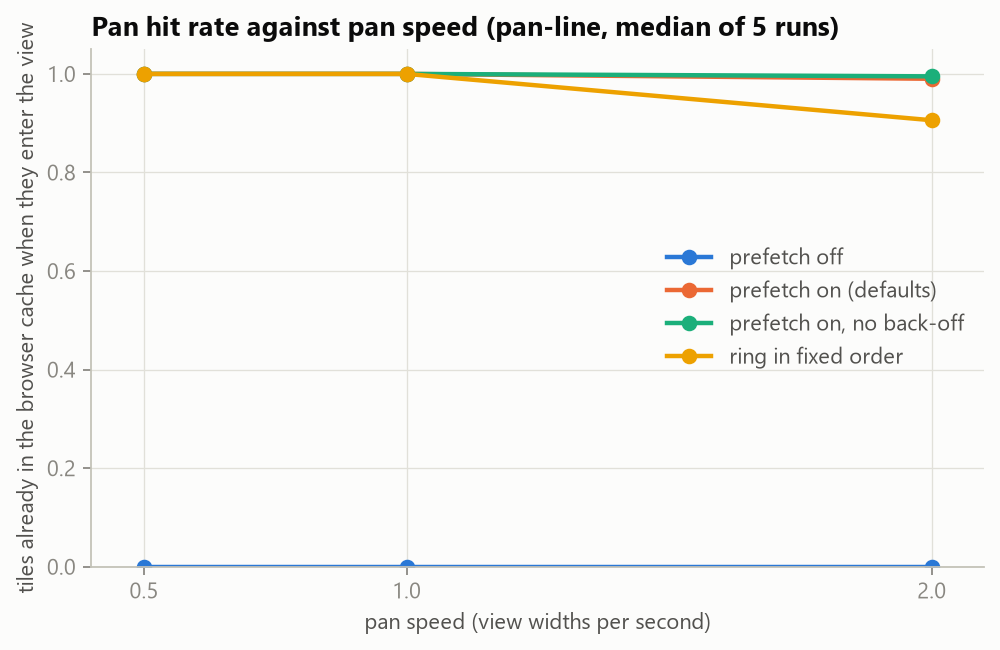
\includegraphics[width=0.66\linewidth]{e6_hit_vs_speed.png}
\caption{Share of tiles already in the browser when they enter the view, straight pans, by pan speed.}
\label{fig:hit}
\end{figure}

\begin{table}[!htbp]
\centering\small
\caption{Prefetch policies over the seven pan traces and zoom-pan (40 runs each; median [interquartile range]).}
\label{tab:prefetch}
\begin{tabularx}{\linewidth}{Xrrrr}
\toprule
Policy & Foreground requests & Pan hit rate & Prefetched & Precision \\
\midrule
prefetch off & 104 [68--135] & 0.30 [0.00--0.51] & 0 & -- \\
defaults (back-off if foreground p95 $>$ 250\,ms) & 0 [0--4] & 1.00 [1.00--1.00] & 218 & 0.34 \\
first policy (back-off at 100\,ms) & 0 [0--56] & 1.00 [0.70--1.00] & 192 & 0.29 \\
no back-off & 0 [0--4] & 1.00 [1.00--1.00] & 232 & 0.34 \\
ring in fixed order & 0 [0--7] & 1.00 [0.97--1.00] & 292 & 0.33 \\
\bottomrule
\end{tabularx}
\end{table}

\begin{itemize}
  \item \textbf{With prefetch} the tiles entering the view during a pan are 98--100\% cached at every speed. The pans
  need 0--5 foreground requests instead of 36--202 (Table~\ref{tab:prefetch}, Figure~\ref{fig:hit}).
  \item \textbf{Without prefetch} the hit rate is 0\% on a straight pan and about 50\% when the pan turns back. The
  view still looks almost complete (blank area-time 0.2--3.4\%), because each new tile arrives in about 50\,ms and
  a coarser level covers the gap.
  \item \textbf{Cost:} the ring fetches 2--5 tiles for each one used (precision 0.20--0.56), since it always loads
  directions the user does not take.
  \item \textbf{Ordering:} loading the direction of travel first keeps the hit rate at 0.99 at two view widths per
  second; a fixed order drops it to 0.91.
  \item \textbf{Back-off threshold:} the first policy stopped prefetch for 2\,s whenever foreground p95 exceeded
  100\,ms. That is the cold-start latency, so prefetch switched off at random, and the fast reversing pan fell to a
  0.50 hit rate. At 250\,ms the policy matches ``no back-off'' everywhere and keeps a safety valve.
\end{itemize}

\subsection{Prefetch and the foreground (gate 1)}
\begin{figure}[!htbp]
\centering
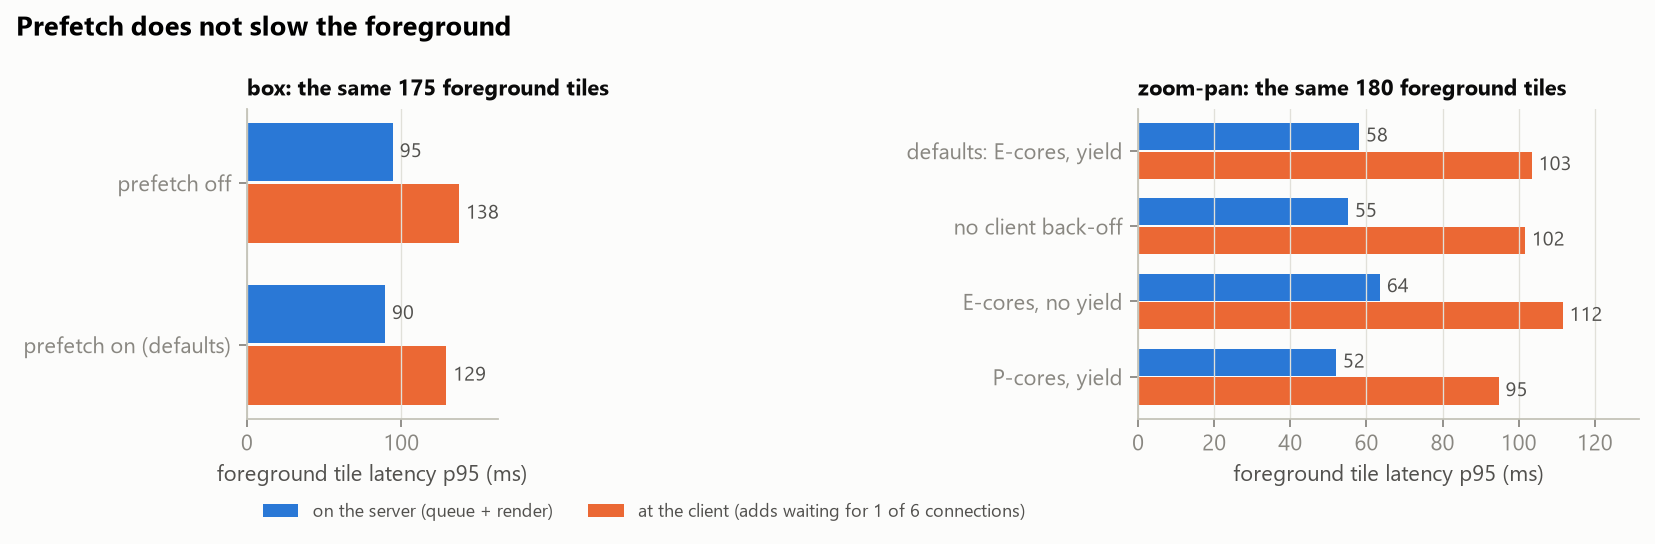
\includegraphics[width=\linewidth]{e6_fg_p95.png}
\caption{Foreground tile latency (95th percentile) on identical tile sets: on the server (queue + render) and at the
client (also waiting for one of six connections).}
\label{fig:fg}
\end{figure}

The gate as specified compares foreground p95 per trace with prefetch on and off. That compares different tiles:
with prefetch on, pans need almost no foreground tiles, and what remains are cold tiles at a new level. The
like-for-like test is the box trace, where the foreground tiles are identical (Figure~\ref{fig:fg}):
\begin{itemize}
  \item \textbf{Result:} server p95 is 90\,ms with prefetch and 95\,ms without; client p95 is 129 vs 138\,ms.
  Prefetch is slightly faster, because it has already decoded shared blocks. The gate passes.
  \item \textbf{Why:} prefetch stops at the first input event of a gesture and restarts only once the view is
  complete. Only 25 of 905 foreground tiles (3\%) were ever requested while a prefetch request was in flight.
  \item \textbf{Placement:} letting prefetch start while foreground work is pending raises server p95 by 9\% on
  zoom-pan.
  \item \textbf{Pinning held throughout:} 20{,}242 foreground jobs ran on performance cores only, and 122{,}215
  prefetch jobs on efficiency cores only.
\end{itemize}

\subsection{Workers, caches and the rest}
\begin{table}[!htbp]
\centering\small
\caption{Mixed traces (pan-walk, zoom-pan, two bursts, box; 25 runs each; medians).}
\label{tab:mixed}
\begin{tabularx}{\linewidth}{lRRRRR}
\toprule
Configuration & Client p95 ms & Server p95 ms & Complete ms & Blocks decoded & Peak RSS MiB \\
\midrule
defaults (8 workers, 1024\,MiB block cache) & 104 & 98 & 260 & 185 & 608 \\
4 / 6 foreground workers & 106 / 101 & 76 / 92 & 254 / 251 & 185 & 588 / 598 \\
no block cache & 146 & 111 & 285 & 1{,}128 & 386 \\
256\,MiB block cache & 108 & 94 & 260 & 185 & 608 \\
result cache off & 103 & 91 & 257 & 185 & 576 \\
slope / aspect & 115 / 115 & 97 / 103 & 255 / 258 & 185 & 606 / 608 \\
precomputed slope & 93 & 56 & 248 & 160 & 562 \\
HMA 8\,m DEM & 118 & 92 & 268 & 130 & 594 \\
OS file cache flushed & 103 & 104 & 257 & 185 & 608 \\
\bottomrule
\end{tabularx}
\end{table}

\begin{itemize}
  \item \textbf{The browser's six connections set the foreground latency.} The client sees about 40\,ms more than
  the server at p95, because tiles wait for a connection. 4, 6 or 8 foreground workers give the same client latency
  (Table~\ref{tab:mixed}); 8 are kept for a second client such as QGIS.
  \item \textbf{The block cache matters:} without it the server decodes 6$\times$ more blocks and p95 rises 40\%.
  256\,MiB suffices for these short traces.
  \item \textbf{The result cache} has no effect within a single fresh session, where no tile is asked for twice. It
  serves repeat visits and several clients.
  \item \textbf{Product, mode and data:} slope and aspect are about 10\% slower than hillshade. Precomputed slope is
  fastest on the server (no halo, no kernel). The 8\,m DEM behaves like the 2\,m one.
  \item \textbf{A flushed OS cache changes nothing:} decoding, not the disk, is the cost, as in Phases 2--4.
\end{itemize}

\subsection{A real browser}
The same traces replayed in headless Chrome, driven in real time over the DevTools protocol, gave:
\begin{itemize}
  \item the same commits, foreground requests (15, 0, 35) and prefetched tiles as the virtual client;
  \item view-complete times within 10\% (298 vs 325\,ms; 123 vs 127\,ms);
  \item first frames 18--25\,ms sooner in Chrome.
\end{itemize}
The simulated latencies are therefore slight upper bounds.

\section{Discussion}
\paragraph{Answers.}
\begin{enumerate}
  \item Yes: computing derivatives on demand keeps up with continuous viewing. Panning is seamless with a ring of
  neighbouring views; the first exact tile after a zoom arrives within about 90\,ms of the commit.
  \item The debounce removes two-thirds of the server's work per zoom gesture, for a fixed wait that 150\,ms keeps
  short while still coalescing a notched wheel.
  \item Prefetch costs efficiency-core time and 2--5 fetched tiles per tile used, but no foreground latency, because
  it never runs while the user is waiting.
  \item The latency that remains comes from the browser's connection limit and from decoding compressed blocks, not
  from computing slope or hillshade. This is the same bottleneck Phases 2--4 found for whole-grid processing.
\end{enumerate}

\paragraph{Limitations.}
\begin{itemize}
  \item One client on one laptop: the result cache and the spare workers serve several clients, which E6 does not
  run.
  \item Short, synthetic traces (1--11\,s): caches never fill, so long sessions are not measured.
  \item Every run starts with an empty server, so a returning user would see faster tiles.
  \item CPU only: Phase 3 predicts little GPU gain at $512\times512$ per tile once the transfer is counted
  (1.3$\times$ including the copies).
\end{itemize}

\section{Next step}
Phase 6 brings Phases 2--5 together in the final report, slides and a recorded demonstration of the viewer and the
QGIS plugin.

\end{document}
